%As with any population we are now seeing an exponential increase of networked devices. This new influx of devices 
%connecting to the Internet is a blessing in some ways, but in others it is a curse. Although the usefulness of the 
%Internet as a marketing tool increases as the number of connected devices does, there is also a dramatically negative
%affect on previously established protocols. One such protocol that is negatively affected by the growth in population 
%on the Internet is the Internet Protocol(IP). The Internet protocol is one of the most fundamental protocols 
%underlying the Internet. It is used in order to assign an address to every device that connects to the Internet. 
%
%The current widely used version of the Internet Protocol is version 4. At the inception of this version of the 
%protocol  

There are both good aspects and bad ones of an increasing network size on the Internet. More devices on the Internet
means that your advertisements will reach a larger audience. It also means you will get more business if 
you are running an on-line shop. But under the hood of the Internet this rapid growth is causing major problems. 


The fundamental standard upon which the Internet is based is known as the Internet Protocol, or IP for short. The IP works by assigning a unique address to every device connected to the Internet. The address assigned to a particular device is that device's IP address. The reason that this protocol exists is to make communication between two devices called the client and the host possible. 


The IP was first introduced in 1981 by DARPA\cite{rfc0791}, based on previous work by Vint Cerf and Bob Khan\cite{1092259}. Back in 1981 it was assumed that an address of 32 bits (1's and 0's) was large enough to assign a unique IP address to all devices connected to the Internet for the foreseeable future. An address of this length can accommodate roughly $2^{32}$ or about 4 billion devices. Unfortunately we live in an age when the number of networked devices is beginning to exceed this limit.


In it's original introduction with the 32-bit addresses IP was widely adopted. The form of IP that was adopted at that point in time was known as the Internet Protocol version 4 (or IPv4). Since then a new form of IP has been proposed\cite{rfc1883}\cite{rfc2460} and deployed in some cases. IPv6 has an address field of 128 bits. This corresponds to approximately $3.4 \times 10^{38}$ addresses. It is estimated that there are about $10^{24}$ stars in the universe, just to put this in perspective.

\begin{figure}[h!]
	\centering
	\title{IPv6 Adoption by Google Registered Domains}
	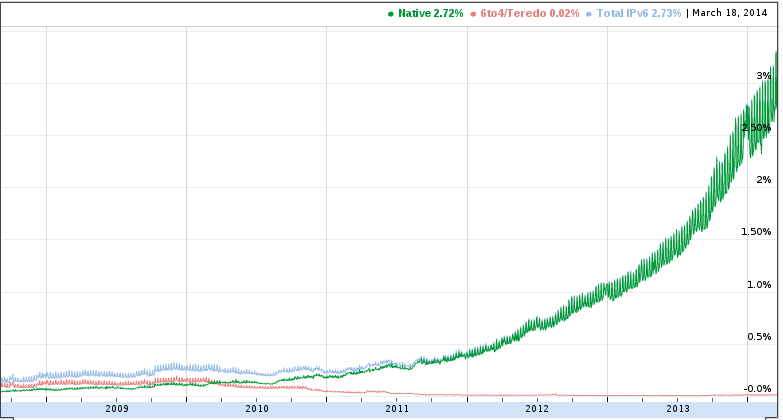
\includegraphics[width = 0.8\textwidth, height = 7cm]{Figures/IPv6Adoption.jpeg}
	\caption{this figure was taken from Google's IPv6 Statistic page\cite{goog}}
\end{figure}

IPv6 has been deployed, but as of March 2014 has only seen a 3.4 \% deployment.\cite{goog} Google takes statistics on domains that register IPv6 addresses in order to monitor the deployment.


The case study we use to exemplify why this Protocol adoption rate can be a problem for businesses was proposed by Lawerence Hughes in his article\cite{sxsc}. We examine the well known company "Skype". Skype is a company that allows its users to make "phone calls" from their computer to any registered phone number (if they buy "Skype Credits"). Unfortunately for Skype, they rely on the old IPv4 and will have a lot of trouble updating their infrastructure to accommodate IPv6. It is understandable that Skype would rely on this older protocol though. IPv4 is widely distributed, and allows Skype to take full advantage of the Internet. This business model, of relying on older protocols is unsustainable but more cost effective initially, and makes entrepreneurs much more cautious of the protocol they choose to rely on. 







   